\documentclass[10pt, a4paper,twocolumn]{article}
% ===== Essential Packages =====
\usepackage[utf8]{inputenc}       % UTF-8 encoding
\usepackage[T1]{fontenc}          % Better font encoding
\usepackage{lmodern}              % Modern Latin Modern font
\usepackage{ctex}                 % Chinese support (must be loaded after fontenc)
\usepackage{subcaption}
% ===== Math & Symbols =====
\usepackage{amsmath}              % Advanced math
\usepackage{amssymb}              % Additional math symbols
\usepackage{mathrsfs}             % Ralph Smith's Formal Script
\usepackage{braket}               % Dirac bra-ket notation
\usepackage{pdfpages}
% ===== Graphics & Tables =====
\usepackage{graphicx}             % Image support
\usepackage{float}                % Better float control
\usepackage{wrapfig}              % Wrapped figures
\usepackage{tikz}                 % Vector graphics
\usepackage[table]{xcolor}        % Colored tables
\usepackage{array}                % Enhanced tables
\usepackage{multirow}             % Multirow tables
\usepackage{tabularx}             % Adjustable-width tables
\usepackage{booktabs}             % Professional table lines
\usepackage{siunitx}              % SI units in tables
\usepackage{caption}              % Better captions
\usepackage{adjustbox}            % Box resizing

% ===== Code Listings =====
\usepackage{listings}             % Code blocks
\usepackage{tcolorbox}            % Colored boxes
\tcbuselibrary{listings, breakable} % Listings in tcolorbox

% ===== Misc =====
\usepackage{lipsum}               % Dummy text
\usepackage{footmisc}             % Better footnotes
\usepackage[margin=1in]{geometry} % Page margins
\usepackage{diagbox}
\usepackage{ctex}
\author{张世航}
\title{阿贝成像和空间滤波}
% ===== 超链接设置 =====
\usepackage{hyperref}
\hypersetup{
	colorlinks=true,
	linkcolor=red,        % 内部链接黑色
	citecolor=blue,         % 引用链接蓝色 <- 修改这里
	urlcolor=red,           % URL链接红色
	filecolor=red,          % 文件链接红色
}

% ===== 附录超链接样式 =====
\usepackage{bookmark}
\bookmarksetup{
	color=red,              % 附录书签红色 <- 修改这里
	bold=false
}
\setlength{\parindent}{0pt}
\begin{document}
    \title{\vspace{-3.5cm}阿贝成像和空间滤波}  % 向上移动标题
    \author{\vspace{-0.5cm}张世航}
    \date{} 
    \maketitle
	\section{$\theta$调制}
	\begin{figure}[H]
		\centering
		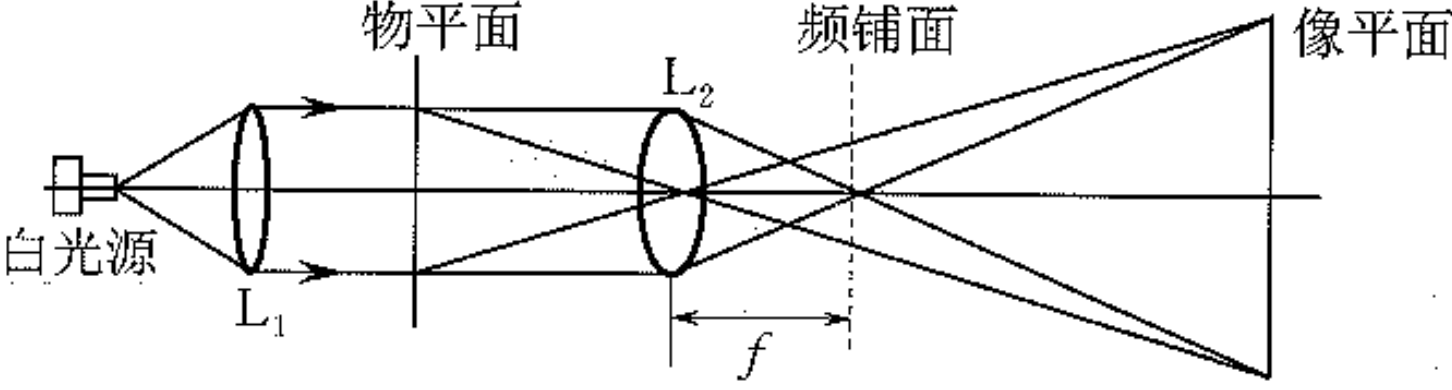
\includegraphics[width=0.7\linewidth]{theta1}
		\caption{}
		\label{fig:theta1}
	\end{figure}	
	\begin{figure}[H]
		\centering
		
\includegraphics[width=0.7\linewidth]{2}
		\caption{天安门1}
		\label{fig:2}
	\end{figure}
	\begin{figure}[H]
		\centering
		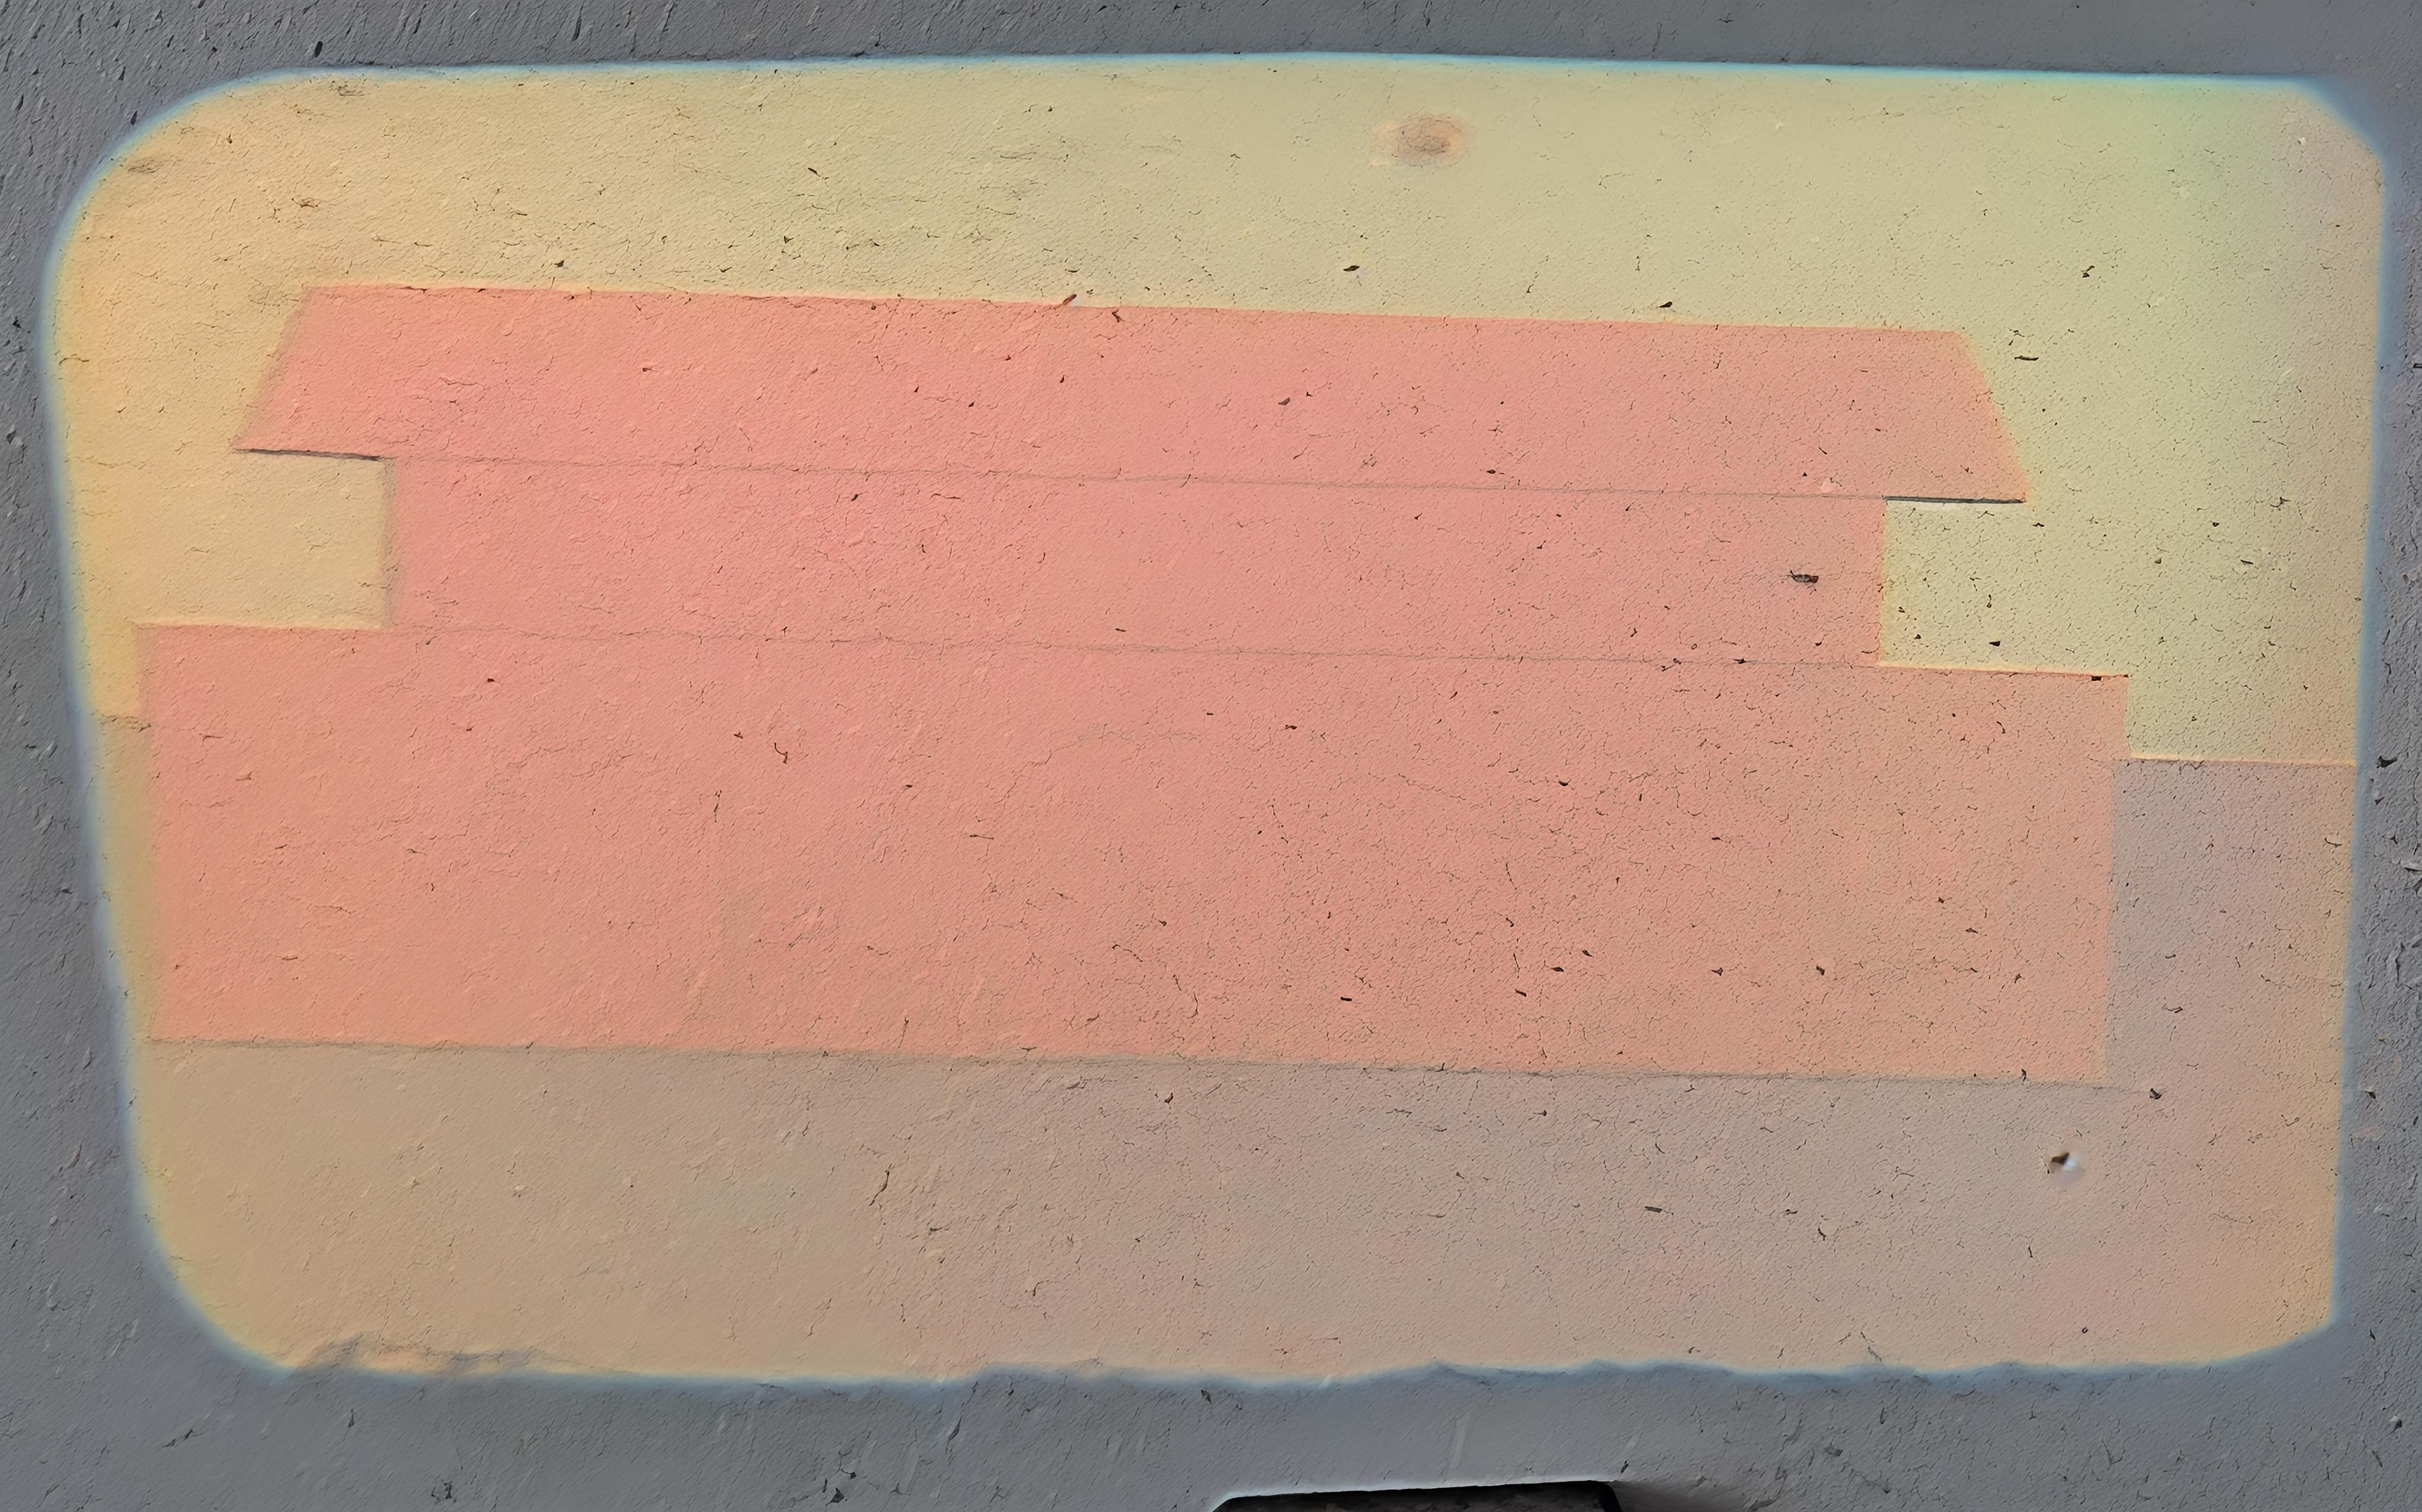
\includegraphics[width=0.7\linewidth]{2.2}
		\caption{天安门2}
		\label{fig:2.2}
	\end{figure}
	\begin{figure}[H]
		\centering
		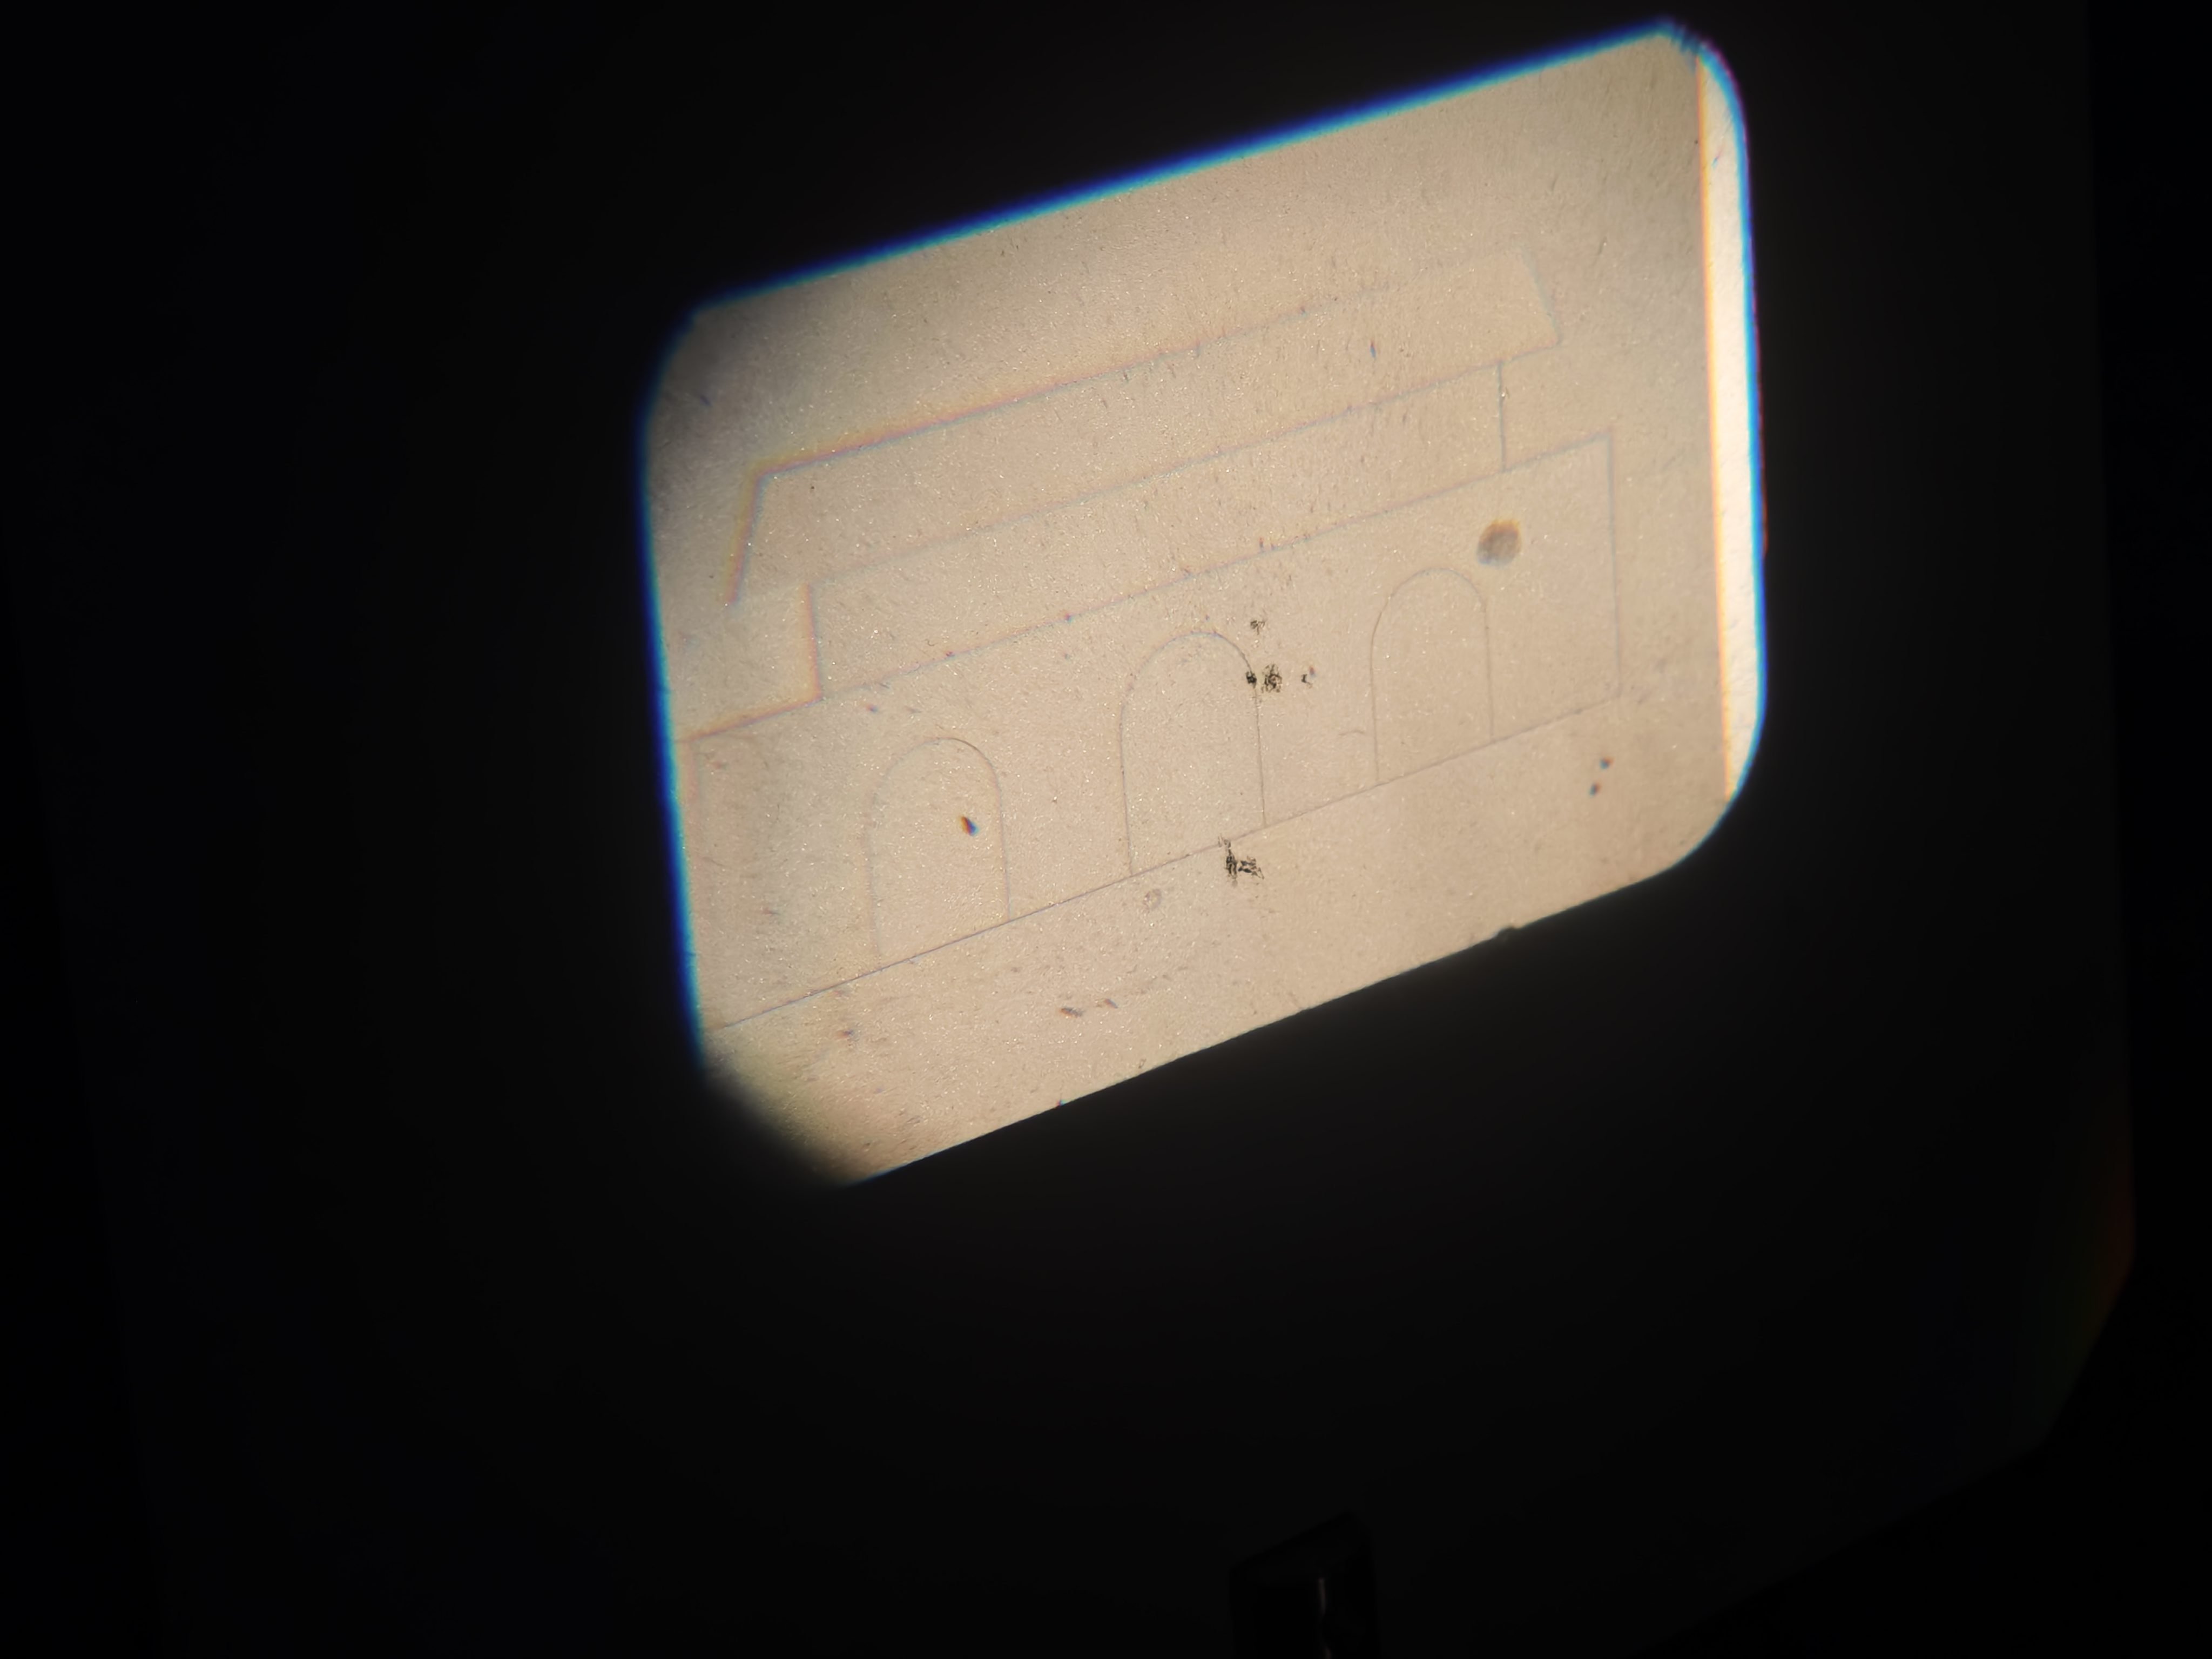
\includegraphics[width=0.7\linewidth]{5}
		\caption{没有颜色的天安门}
		\label{fig:5}
	\end{figure}


	\section{阿贝—波特实验}
	\begin{figure}[H]
		\centering
		
\includegraphics[width=0.7\linewidth]{bote}
		\caption{阿贝—波特实验}
		\label{fig:bote}
	\end{figure}
	
	光栅透过率为\[t(x_1)=[rect(\frac{x_1}{a}*\frac{1}{d}comb(\frac{x_1}{d}))]rect(\frac{x_1}{L})\]
	如\ref{fig:bote}所示,在$P_2$上.\\
	\begin{align*}
		T(f_x)&=\frac{aL}{d}\sum_{n=-\infty}^{\infty}sinc(\frac{an}{d})sinc[L(f_x-\frac{n}{d})]\\
		&=\frac{aL}{d}\{sinc(Lf_x)+sinc(\frac{a}{d})sinc(\frac{a}{d})sinc[L(f_x-\frac{1}{d})]\\&+sinc(\frac{a}{d})sinc[L(f_x+\frac{1}{d})]+\ldots\}
	\end{align*}
	即产生\ref{fig:1},紧靠狭缝后的透射光场为
	\[T(f_x)H(f_x)=\frac{aL}{d}sinc(Lf_x)\]
	在\ref{fig:bote}中的$P_3$面输出的光场.\\
	\begin{figure}[H]
		\centering
		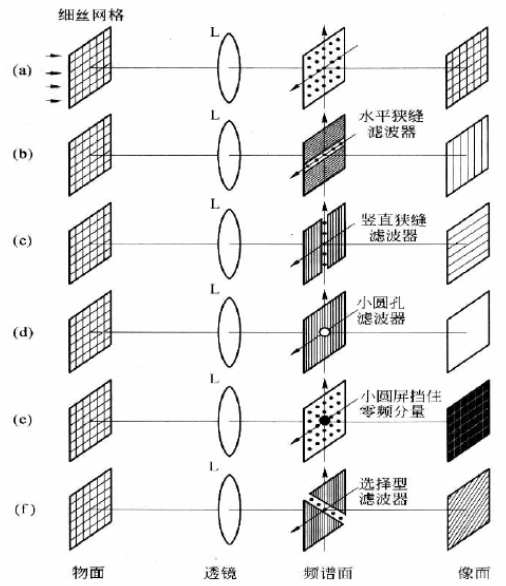
\includegraphics[width=0.7\linewidth]{any}
		\caption{各种滤波器}
		\label{fig:any}
	\end{figure}
	

       
	\subsection{阵列图样}
	\begin{figure}[H]
		\centering
		
\includegraphics[width=0.7\linewidth]{1}
		\caption{二维光点阵列}
		\label{fig:1}
	\end{figure}
	\subsection{条纹图样}
	\subsubsection{点阵频谱}
	我们在\ref{fig:bote}的$P_2$使用点阵频谱面得到方格条纹\ref{fig:6}
	\begin{figure}[H]
		\centering
		
\includegraphics[width=0.7\linewidth]{6}
		\caption{方格条纹}
		\label{fig:6}
	\end{figure}
	\subsubsection{竖直狭缝}
	我们使用竖直狭缝得到水平条纹\ref{fig:7}.如\ref{fig:any}的(c)所示.\\
	\begin{figure}[H]
		\centering
		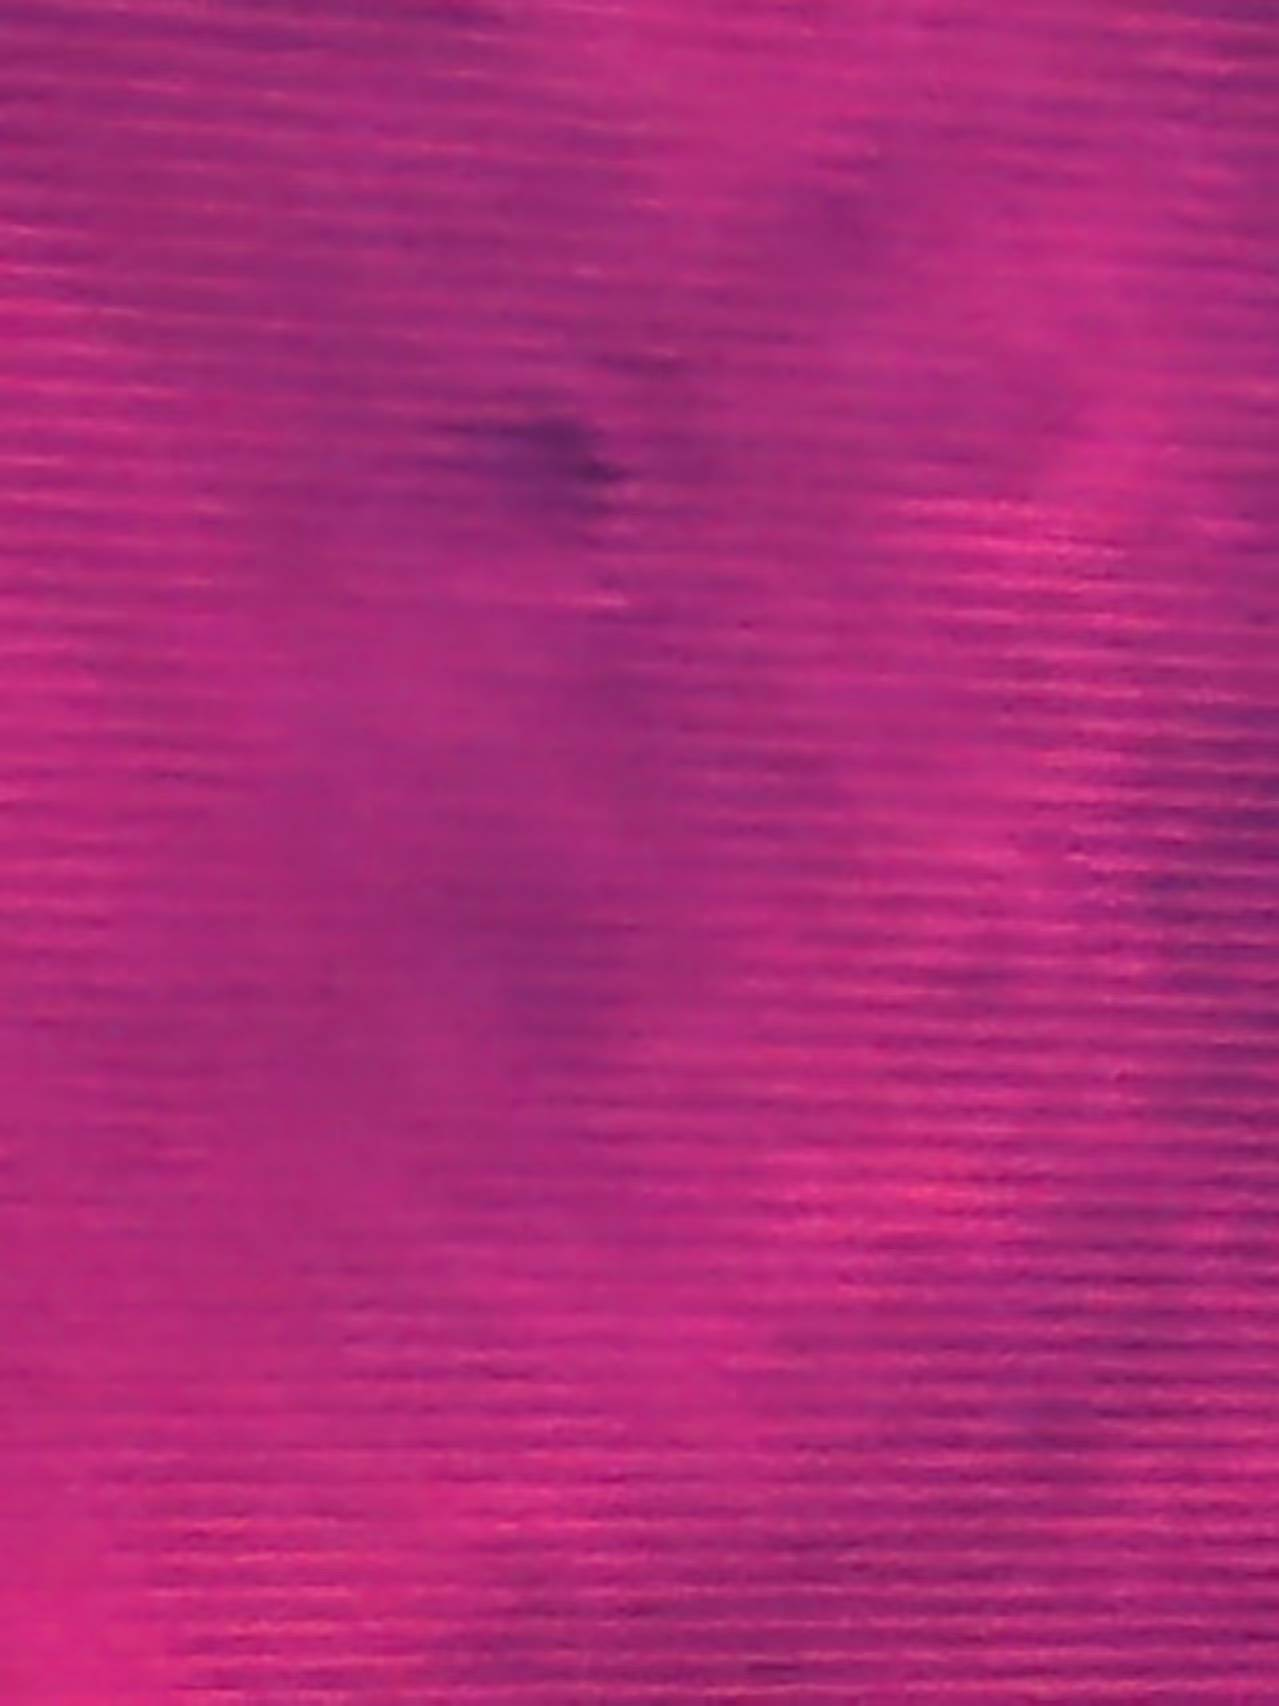
\includegraphics[width=0.6\linewidth]{7}
		\caption{水平条纹}
		\label{fig:7}
	\end{figure}
	\subsubsection{水平狭缝}
	我们使用水平狭缝得到下图的竖直条纹\ref{fig:8}.如\ref{fig:any}的(b)所示.
	\begin{figure}[H]
		\centering
		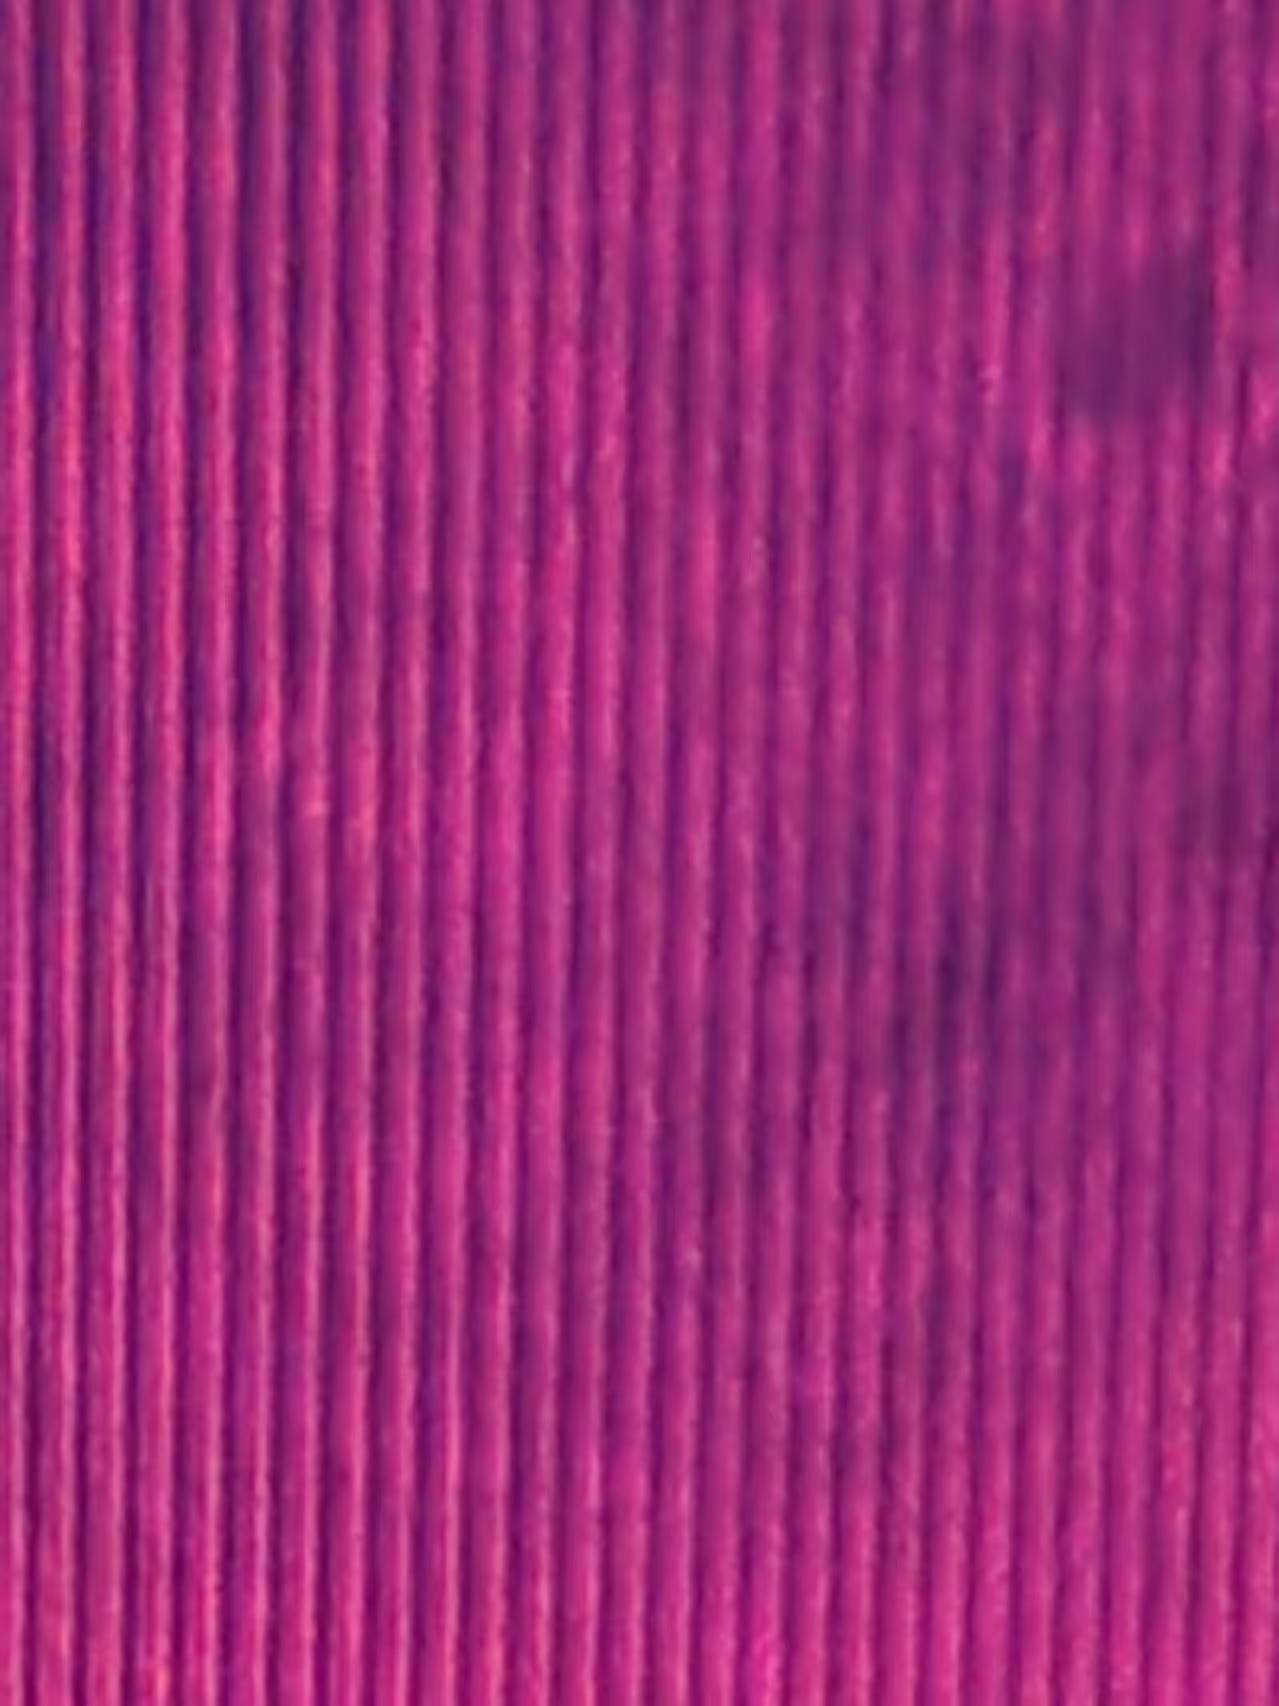
\includegraphics[width=0.6\linewidth]{8}
		\caption{竖直条纹}
		\label{fig:8}
	\end{figure}
	\subsubsection{倾斜狭缝}
	我们使用斜着的条纹得到反方向倾斜的条纹\ref{fig:9}.如\ref{fig:any}的(f)所示.\\
	\begin{figure}[H]
		\centering
		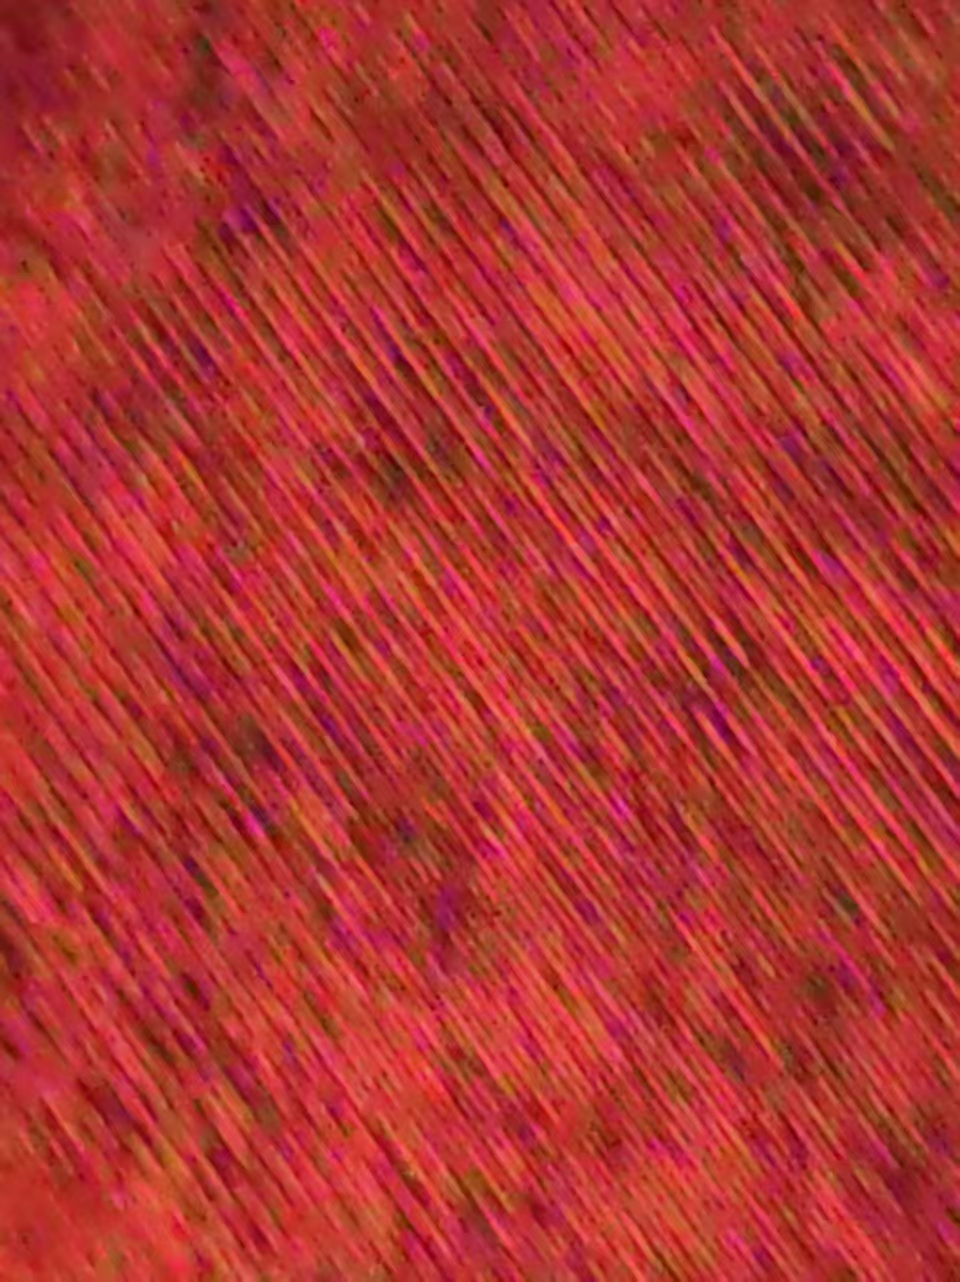
\includegraphics[width=0.6\linewidth]{9}
		\caption{斜条纹}
		\label{fig:9}
	\end{figure}
	利用空间滤波技术可以成功的改变图像的结构.
	\section{相干滤波}
	\begin{figure}[H]
		\centering
		
\includegraphics[width=0.7\linewidth]{lvbo}
		\caption{二元振幅滤波器}
		\label{fig:lvbo}
	\end{figure}
	
	\subsection{低通滤波—消除图像上周期性网格}
	\begin{figure}[H]
		\centering
		
\includegraphics[width=0.7\linewidth]{din}
		\caption{低通滤波}
		\label{fig:din}
	\end{figure}
	网点图像复振幅分布:\[f_s(x_1,y_1)=comb(\frac{x_1}{y_1})comb(\frac{y_1}{Y})f(x_1,y_1)\]
	{\color{blue}comb函数表示周期性的采样结构(网格)}\\
	{\color{blue}$f(x_1,y_1)$是原始图像(如\ref{fig:11}})\\
	{\color{blue}X,Y是网格在x和y方向上的周期}\\
	经过傅里叶变换,频谱面上得到:\[F_s(f_x,f_y)=XYcomb(Xf_x)comb(Yf_y)\otimes F(f_x,f_y)\]
	{\color{blue}$F(f_x,f_y)$是原始图像的频谱.}\\
	{\color{blue}$comb(Xf_x)⋅comb(Yf_y)$表示网格的频谱,是一个在频率空间中的周期性点阵.}\\
	{\color{blue}“$\otimes$”表示卷积,意味着原始图像的频谱在频率域中被周期性复制.}\\
	\subsubsection{有方格的光-未滤波}
	\begin{figure}[H]
		\centering
		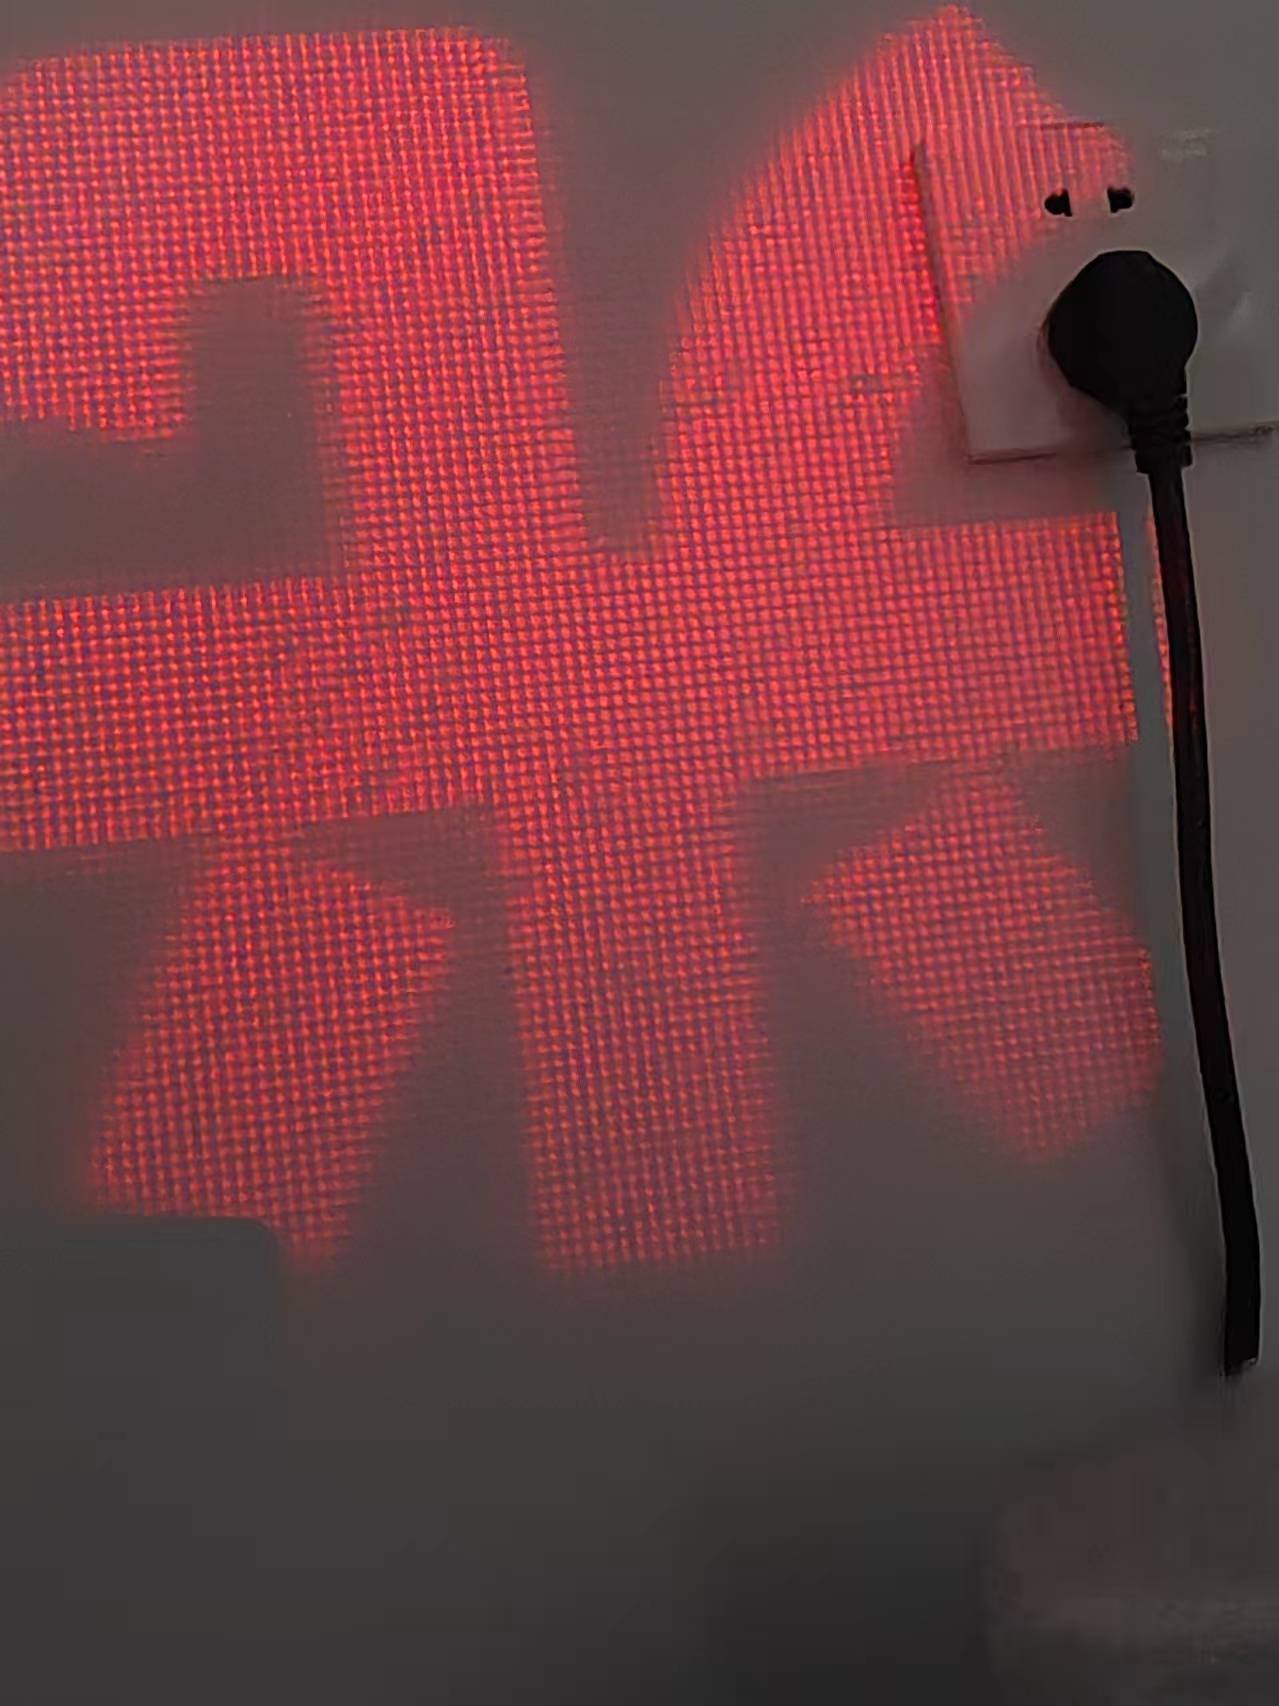
\includegraphics[width=0.6\linewidth]{11}
		\caption{有方格的光}
		\label{fig:11}
	\end{figure}
	网格的周期性结构(高频)与文字的连续结构(低频)同时成像,因此图像上既有文字也有网格.\\
	\subsubsection{没有方格的光—滤波}
	\begin{figure}[H]
		\centering
		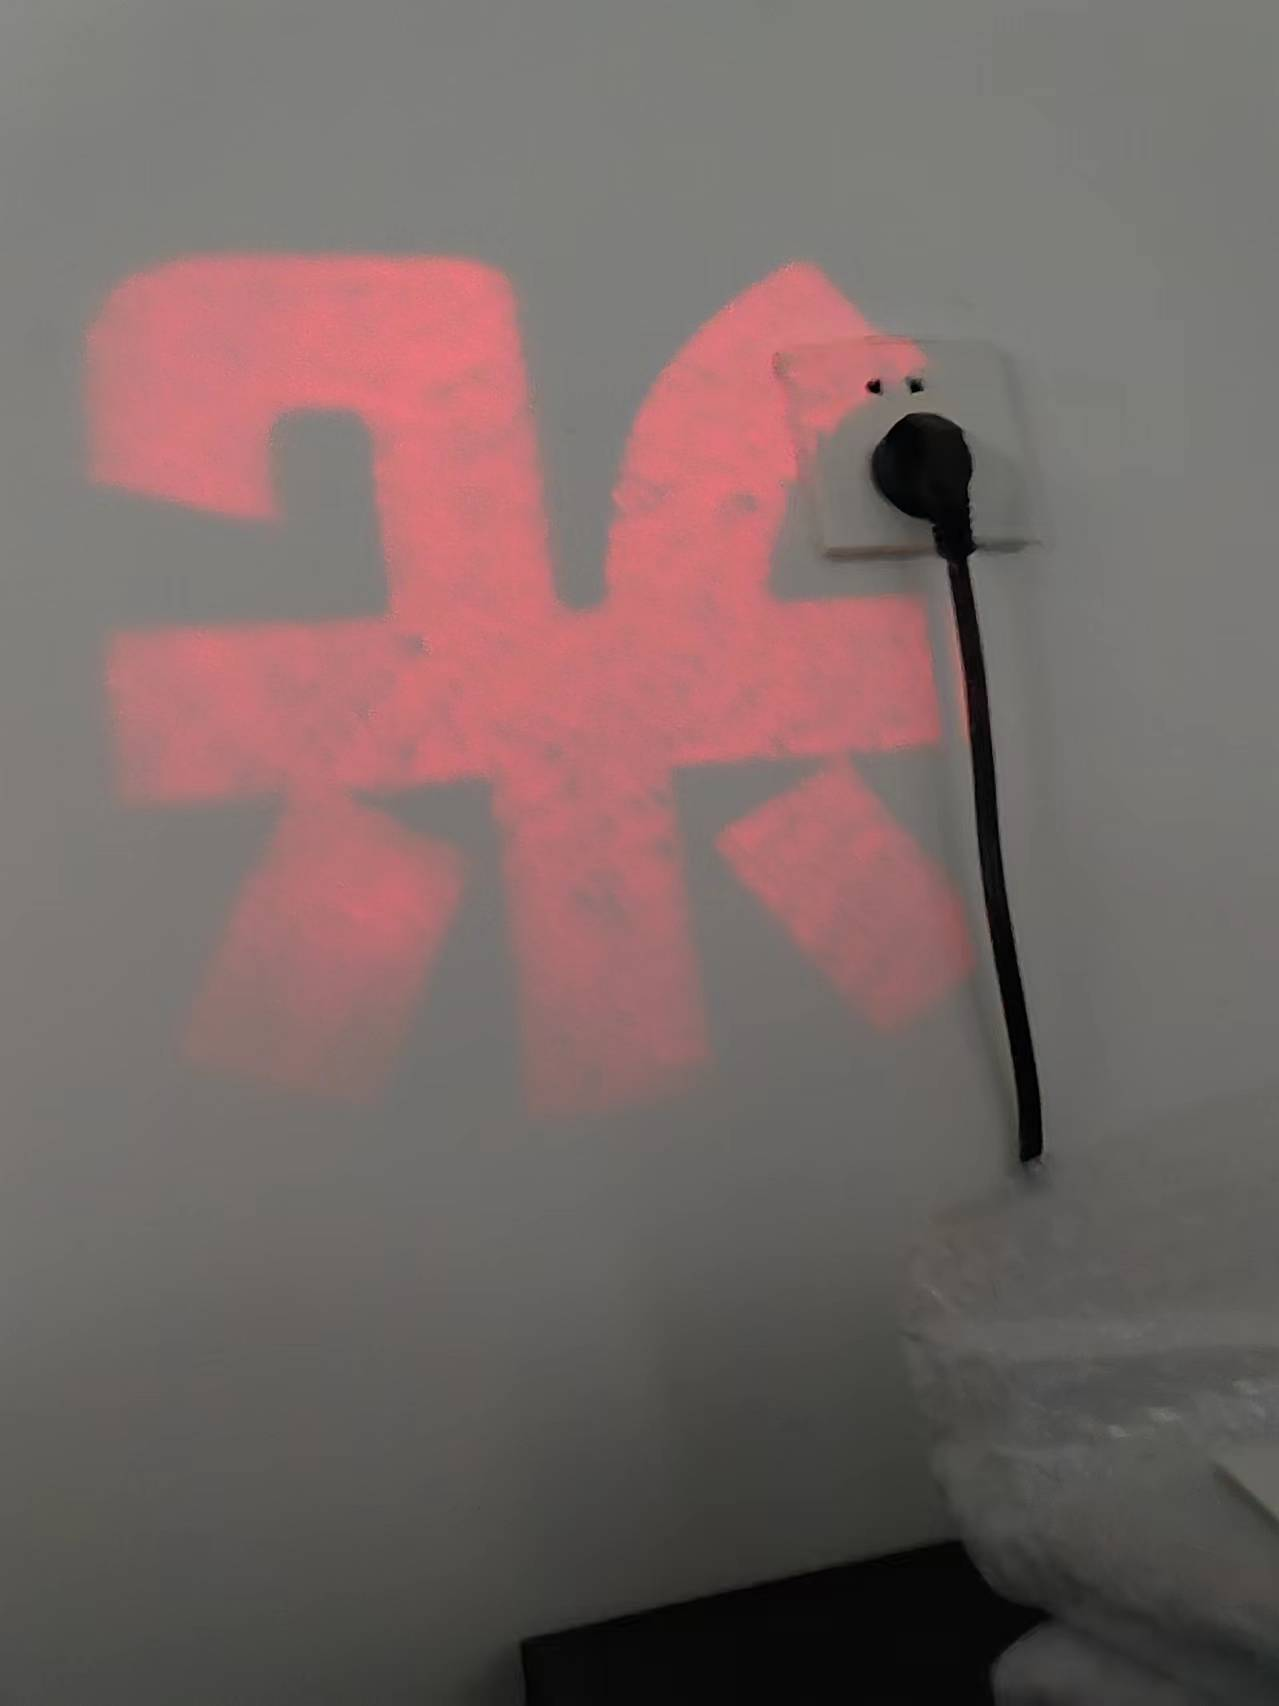
\includegraphics[width=0.6\linewidth]{10}
		\caption{没有方格的光}
		\label{fig:10}
	\end{figure}
	未放置\ref{fig:lvbo}的a的时候成像为\ref{fig:11}.放置\ref{fig:lvbo}的a,在像面上,网格的高频信息消失,网格图案被“抹掉”;而文字的低频信息被保留,仍然成像.如\ref{fig:10}所示.
	\subsection{高通滤波——用于增强边缘}
	\subsubsection{没有边界的"十"字-未滤波}
	\begin{figure}[H]
		\centering
		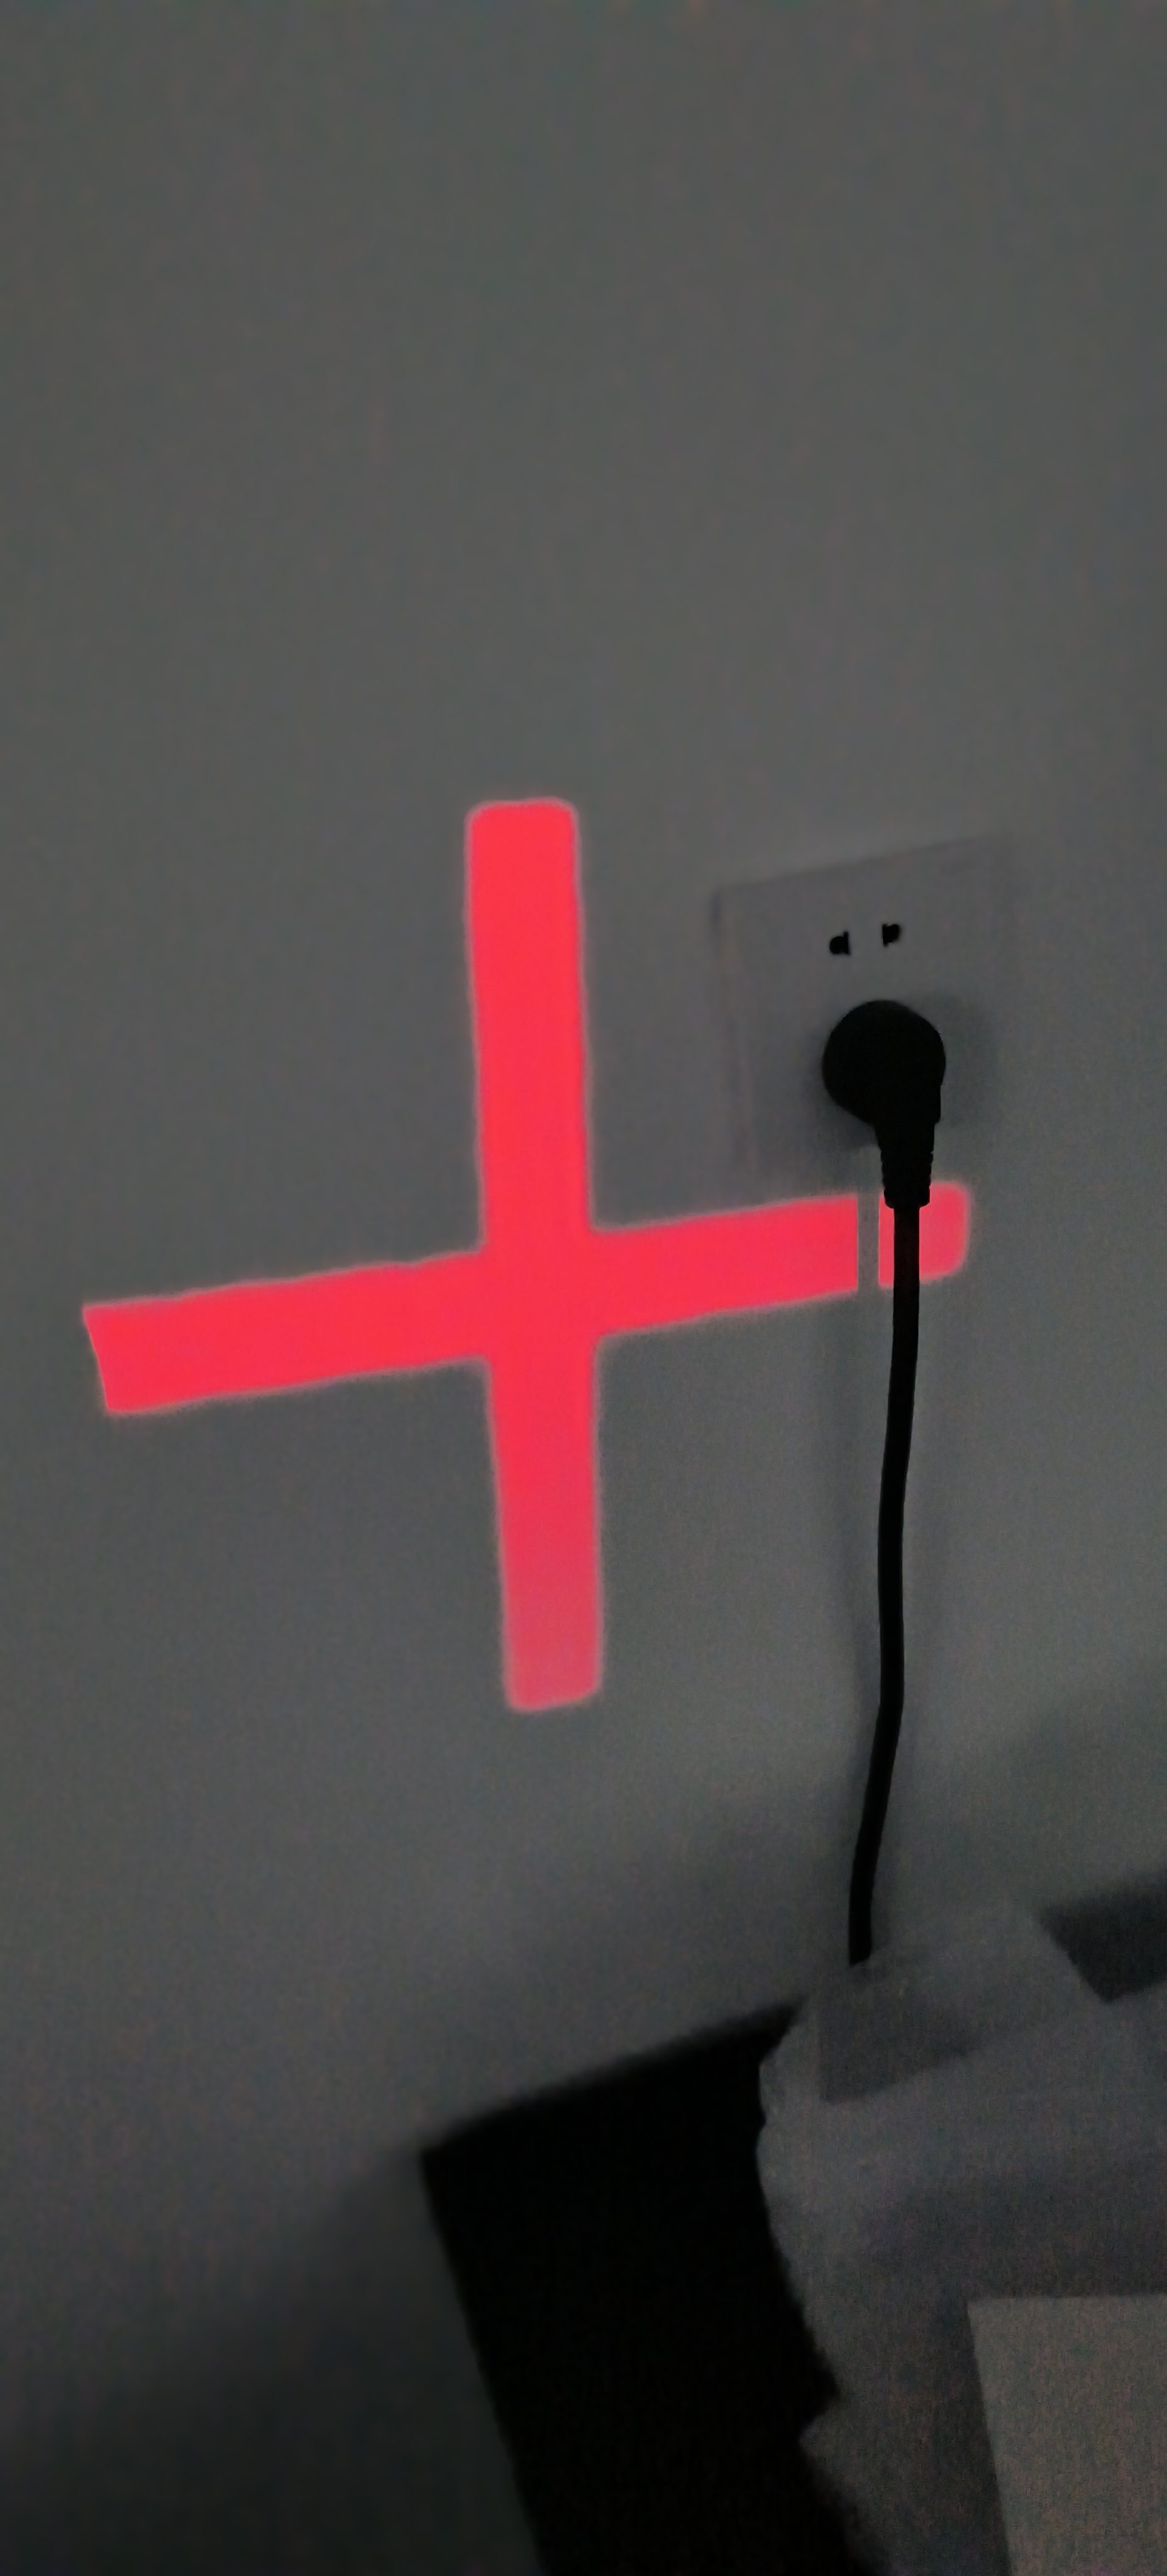
\includegraphics[width=0.5\linewidth]{15}
		\caption{没有边界的"十"字}
		\label{fig:4}
	\end{figure}
	图像\ref{fig:4}看起来模糊,没有明显边界,是因为它主要包含低频信息,缺乏高频的边缘细节.\\
	\subsubsection{有边界的"十"字—滤波}
	\begin{figure}[H]
		\centering
		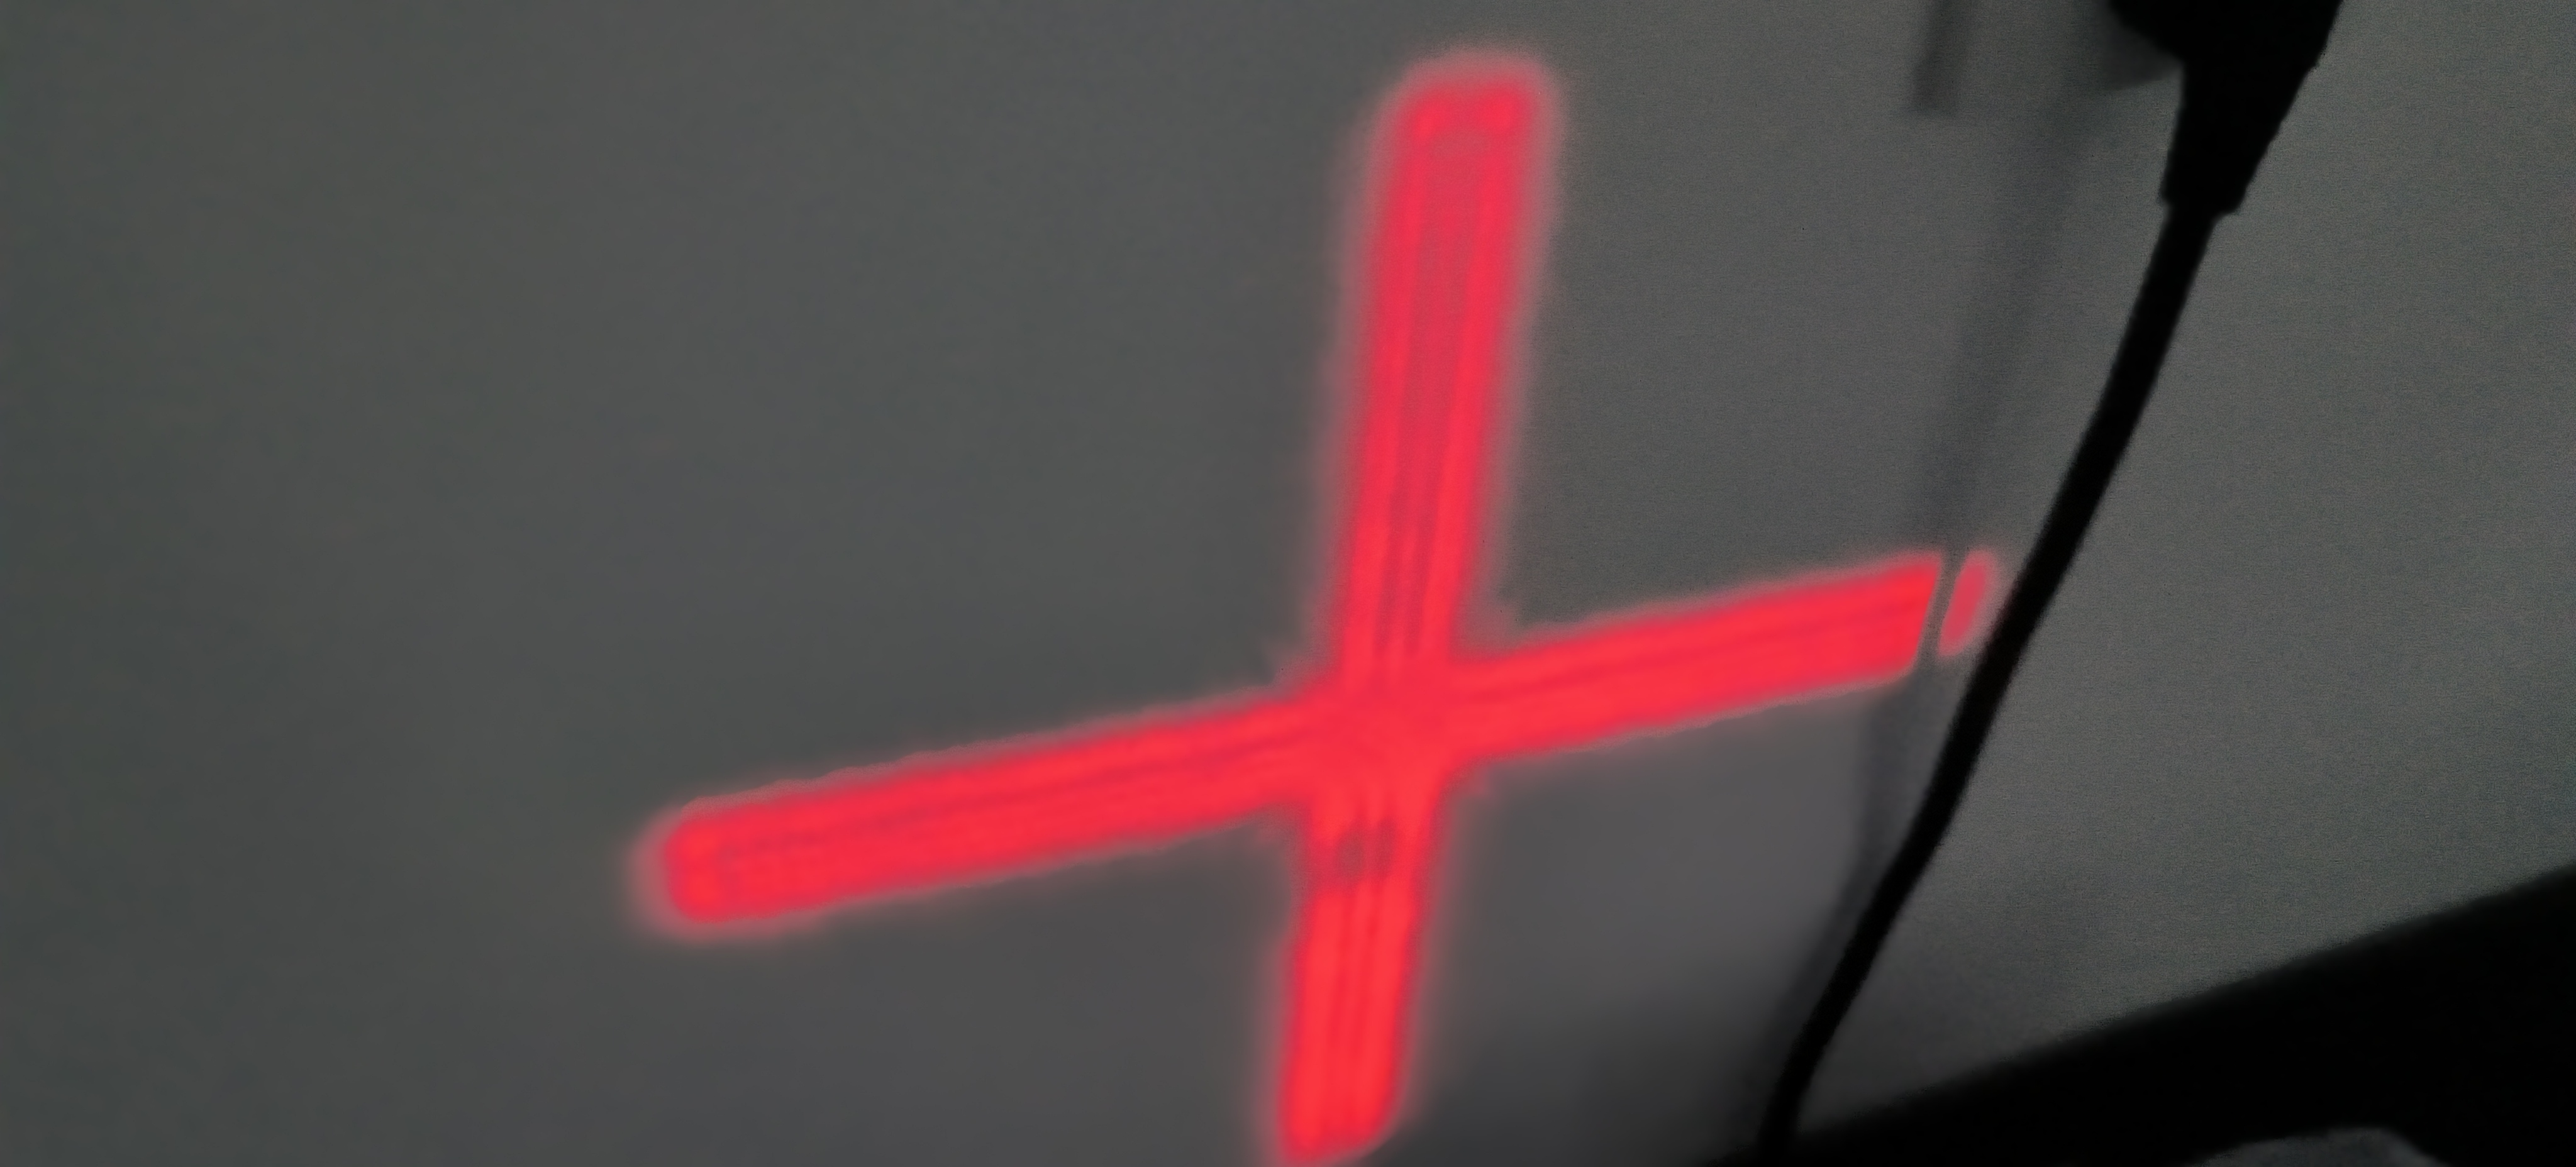
\includegraphics[width=0.7\linewidth]{3}
		\caption{有边界的"十"字}
		\label{fig:3}
	\end{figure}
	图像\ref{fig:3}中高通滤波器阻挡了中心低频光，只让高频光通过,导致图像中的大面积均匀区域（低频）变暗或消失,图像的边缘部分(高频)被突出显示,因此“+”字的边界变得清晰可见.\\
	
	
		
	网格的频谱:网格是周期结构,其空间频率是离散的,对应的频谱是分立的高频亮点(分布在频谱面的特定位置).
	字样的频谱:字样是非周期结构,其空间频率是连续的,对应的频谱是从低频(中心)到高频(边缘)的连续分布(低频分量决定字样的整体轮廓,高频分量决定细节).
	高通滤波器是一个中心带不透明小圆屏的透明膜片(如\ref{fig:lvbo}的b所示),其功能在于滤去低频成分,以增强像的边缘,提高对模糊图像的识别能力,或实现对比度的反转.\\
	
	

	
\end{document}